\documentclass[11pt]{article}

\usepackage[margin=1in]{geometry}
\usepackage{amsmath,amssymb}
\usepackage{booktabs}
\usepackage{graphicx}
\usepackage{natbib}
\usepackage{hyperref}
\usepackage{xcolor}
\hypersetup{colorlinks=true, linkcolor=black, citecolor=black, urlcolor=blue}

\title{Do prediction intervals for satellite-based poverty estimates
survive a national border? A pre-registered evaluation in West Africa}

\author{Abdoulie Balisa\\
Department of Statistics and Actuarial Science\\
Kwame Nkrumah University of Science and Technology\\
\texttt{abalisa@st.knust.edu.gh}}

\date{August 2026}

\begin{document}
\maketitle

\begin{abstract}
Satellite-based models of household wealth are trained and validated on survey
clusters from one set of countries and then applied to countries with no survey
at all. Their reported accuracy is therefore measured under conditions that do
not match how they are used. We asked whether the uncertainty such models report
remains valid across a national border, using cluster-level wealth index values
from twelve West African Demographic and Health Surveys (6{,}706 clusters,
155{,}796 households) and open geospatial covariates. The Gambia was withheld
from every stage of model development and evaluated once, against a threshold
registered in advance.

Four hypotheses were stated before analysis and none was supported. Point
accuracy degraded by about three per cent across a border rather than the
predicted third ($R^2 = 0.746$ in-country under spatial blocking, $0.723$ under
leave-one-country-out, $0.673$ on The Gambia). Mean conformal coverage also
transferred: a nominal 90\% interval covered 88.7\% of held-out foreign clusters
and 89.3\% of Gambian clusters, where the pre-registered prediction was
substantially less than 90\%. Correlation alignment degraded point accuracy
rather than improving it. The pre-registered target-country test of a
coverage-reliability hypothesis returned a null at 53\% power.

The average is nonetheless the wrong summary, and this is the paper's clearest
result. Coverage for an individual held-out country is dispersed by 2.8 to 4.7
times what sampling variation permits, at every nominal level tested
($\chi^2_{10}$ from 108.9 to 273.1, $p < 10^{-17}$ throughout), ranging from
0.821 to 0.979 at nominal 90\%. The same procedure that covers 82\% of
Mauritanian clusters covers 98\% of Togolese ones, and nothing observable in
advance separates the two cases. Dispersion also grows as the nominal level
falls, so intervals are least trustworthy where they are narrowest. The Gambia
falls within 1.1 standard deviations of that distribution at every level, an
unremarkable draw from a wide spread rather than a well-calibrated case. A
practitioner deploys to one country, so this dispersion rather than the mean is
the operationally relevant quantity, and it is invisible to any evaluation that
pools countries. A secondary comparison suggesting that constant-width intervals
fail in shape where adaptive ones do not was tested against the eleven training
countries, did not replicate, and is reported as withdrawn.
\end{abstract}

\section{Introduction}

Household surveys are expensive and infrequent. The Gambia has two Demographic
and Health Surveys with georeferenced clusters, in 2013 and 2019--20. Many
countries have fewer. The standard response is to train a model that predicts
survey-measured wealth from satellite imagery and other open geospatial data in
countries where surveys exist, then apply it where they do not
\citep{jean2016,yeh2020,chi2022}.

The published literature reports how accurate such models are. It reports this
almost always by holding out clusters from the same countries used for training.
The application of interest is different: a country with no survey at all. If
accuracy is estimated in-domain and the model is applied out-of-domain, reported
performance may not describe the deployment setting.

Point accuracy under this shift is reasonably well studied. \citet{yeh2020}
report $R^2 = 0.67$ for asset wealth in held-out countries. Uncertainty is
treated less consistently. Interval estimates are sometimes published:
\citet{chi2022} release a confidence interval with every wealth microestimate,
and \citet{kakooei2024} study predictive uncertainty for poverty estimation
explicitly under cross-country transfer. Empirical calibration is reported
rarely and narrowly. \citet{chi2022} construct intervals from a regression on
absolute residuals, note its limited explanatory power, and do not report the
coverage those intervals achieve. In concurrent work, \citet{olanrewaju2026} do
report coverage, at 88.4\% against a 90\% target, for estimates fitted on each
country's own survey. That is one figure at one nominal level for the in-country
regime, and it is the closest published check we found.

A model that predicts a cluster's wealth index and attaches a 90\% prediction
interval makes a falsifiable claim: across many such clusters, 90\% should
contain the truth. We measure whether that claim holds, and whether it survives
a national border.

This paper measures it. The contribution is the measurement and the design that
makes it interpretable, not the direction of the answer, which was not what we
predicted.

\subsection{What we predicted, and what happened}

Four hypotheses were fixed before data access was granted, in a protocol
committed to version control (Section~\ref{sec:preregistration}). All four were
disconfirmed. We report this rather than reframing it, and Section~\ref{sec:res}
gives each result at the strength the evidence supports.

\section{Related work}

\subsection{Predicting wealth from satellite and digital trace data}

The modern form of this problem was set by \citet{jean2016}, who used transfer
learning from nighttime lights to extract features from daytime satellite
imagery and predicted cluster-level consumption and assets in five African
countries, reporting $R^2$ up to 0.56. \citet{yeh2020} scaled the approach to
roughly 20{,}000 villages across 23 African countries with a multispectral
convolutional network, reporting $R^2 = 0.67$ for asset wealth in held-out
countries, which remains the strongest published evidence that point accuracy
survives a border.

Cross-country prediction has been examined directly. \citet{lee2022} build
village-level poverty maps across 25 sub-Saharan African countries and evaluate
prediction for one country from others. \citet{corral2025} assess how these
models behave where no survey exists and find the errors are not random. The
direction of the error tracks the characteristics of the place: living standards
come out too high where the area is poor, rural or dependent on one sector, and
too low where it is richer and more urban. Adding spatial structure to the model
does not remove the pattern. Their finding
concerns the location of the point estimate. Ours concerns the width of the
interval around it, and the two are complementary: a biased point estimate with
an honest interval and an unbiased one with a dishonest interval fail a
decision-maker in different ways.

A parallel line uses digital trace data. \citet{blumenstock2015} predicted
wealth from mobile phone metadata in Rwanda, and \citet{chi2022} drew on
several data sources at once, among them satellite imagery, mobile network
records, topography and aggregated connectivity, to release wealth
microestimates covering every low- and middle-income country at 2.4\,km
resolution. Their training data came from surveys in 56 countries, with
accuracy checked in 18 more. \citet{smythe2022} used high-resolution poverty
maps of this kind for geographic targeting of social assistance, which is the
application that makes the reliability of these estimates consequential rather
than academic.

Across this literature, headline performance is reported as $R^2$ or rank
correlation. Uncertainty is not ignored. \citet{chi2022} publish a confidence
interval for every microestimate, deriving it from a linear regression on
absolute residuals, and are explicit that this regression has limited
explanatory power ($R^2 = 0.09$ under spatially stratified cross-validation).
\citet{kakooei2024} go further in our direction, quantifying predictive
uncertainty from deep learning and evaluating which source countries to train
on when predicting a target country, which is the same transfer setting we
study.

One study closes that loop, concurrently with ours. \citet{olanrewaju2026}
build relative wealth estimates for 23 African countries from open data,
evaluate cross-country transfer at $R^2 = 0.62$ under leave-one-country-out, and
report that their split-conformal intervals attain 88.4\% coverage against a
90\% target. That coverage figure accompanies estimates fitted on each country's
own survey, and their transfer analysis reports point accuracy without a
matching coverage figure.

A closer methodological neighbour is \citet{adjei2026}, who fuse satellite and
reanalysis data to map PM2.5 across 29 African countries, validate under
location-grouped spatial cross-validation, and apply split conformal prediction
at a nominal 90\% level. They report empirical coverage and find it fails
badly under geographic shift, at 65.3\% against the 90\% target in East Africa,
which they attribute to covariate shift measured directly. The outcome variable
is air quality rather than welfare, the shift is regional rather than across a
national border, and coverage is reported at one nominal level for one region.
Their result nonetheless matters here, because it establishes that conformal
coverage on African satellite products can collapse under spatial shift. Our
finding that it largely holds is therefore a contrast to be explained rather
than a foregone conclusion, and we return to it in Section~\ref{sec:disc}.

What remains unmeasured is therefore not whether these intervals are calibrated
at all, but whether calibration survives the border for this outcome. Establishing that requires
coverage in-country and out-of-country for the same model and the same
calibration set, resolved per country rather than pooled, and at more than one
nominal level, since a method can hold at 90\% while failing at 50\%. We report
all three, with the target country held back for a single pre-registered test.
Where our figures and theirs are comparable they agree closely, which we read as
independent corroboration rather than as a discrepancy to explain.

\subsection{Small area estimation, where coverage is validated}

There is a separate tradition in which interval calibration is standard.
Model-based small area estimation combines survey data with auxiliary
covariates and reports mean squared error and interval coverage as a matter of
course, and it has increasingly used geospatial and satellite covariates for
poverty and wealth \citep{masaki2020,newhouse2023,permatasari2025}. Coverage in
that literature is typically established by design-based simulation or by
comparison against a census, in settings where the model is applied within the
country whose survey trained it.

Our question is what happens to a distribution-free interval when the model is
carried across a border into a country with no survey at all, which is the
regime the satellite-based literature actually targets and the one small area
estimation is not usually asked to serve. We take the practice of validating
coverage from that tradition and apply it in this one.

\subsection{Validation under spatial dependence}

Survey clusters near one another share covariates, so a random train/test split
places near neighbours on both sides and inflates measured accuracy.
\citet{roberts2017} survey blocking schemes for data
carrying spatial, temporal, hierarchical or phylogenetic dependence. Their
recommendation is stronger than it first appears: blocking should be used
whenever the design implies dependence, and a model whose residuals look
uncorrelated is not evidence that it can be skipped. \citet{ploton2020} give a case where the
correction is not marginal. Mapping forest biomass in central Africa, they
report that the usual random-split figure credited the model with explaining
over half the variation, and that once folds were separated in space almost none
of that apparent skill remained.

The reason this bears on our design is specific. Our central comparison is between
in-country and out-of-country performance, so an inflated in-country baseline
would manufacture the effect we set out to measure. We therefore block all
within-country validation and report the naive figure alongside, so the size of
the correction is visible.

\subsection{Conformal prediction and distribution shift}

Conformal prediction \citep{vovk2005} constructs prediction sets with
finite-sample marginal coverage for any underlying model, requiring only that
calibration and test data be exchangeable. \citet{romano2019} introduced
conformalized quantile regression, which conformalises the output of quantile
models so that interval width varies with the input rather than being constant
across the covariate space.

The exchangeability requirement is exactly what cross-border transfer violates.
\citet{tibshirani2019} generalised conformal prediction to weighted
exchangeability, showing that valid coverage can be recovered under covariate
shift when the density ratio between source and target is known or estimable.
\citet{barber2023} analysed the non-exchangeable case more broadly and bounded
the coverage gap in terms of the distribution shift.

That theory tells us coverage \emph{can} fail under shift and how it might be
repaired. It does not say how much coverage is actually lost when a poverty
model crosses a West African border, which is an empirical quantity. Measuring
it is the contribution here. We deliberately use unweighted conformal
prediction rather than the weighted correction of \citet{tibshirani2019},
because the question is what happens to the guarantee as it is ordinarily
applied, not whether a correction exists.

\subsection{Domain adaptation}

Methods that align source and target feature distributions are the standard
response to covariate shift. We use CORAL \citep{sun2016}, which matches
second-order statistics between domains by a linear transformation and requires
target features but no target labels. Its relevance to this paper is that
distribution alignment operates on features and has no mechanism acting on
interval width, which motivated our third hypothesis.

\section{Data}

\subsection{Surveys}

Twelve West African DHS surveys, listed in Table~\ref{tab:surveys}. The unit of
analysis is the DHS cluster, an enumeration area, which is the finest spatial
unit at which wealth is released. The label is the cluster mean of \texttt{hv271},
the DHS wealth index factor score.

\begin{table}[t]
\centering
\small
\begin{tabular}{llrrr}
\toprule
Country & Survey & Year used & Clusters & Households \\
\midrule
The Gambia (target) & 2019--20 & 2020 & 280 & 6{,}549 \\
Senegal & 2019 Continuous & 2019 & 214 & 4{,}538 \\
Mali & 2018 & 2018 & 328 & 9{,}510 \\
Nigeria & 2018 & 2018 & 1{,}382 & 40{,}427 \\
Ghana & 2014 & 2014 & 423 & 11{,}835 \\
Burkina Faso & 2021 & 2021 & 514 & 13{,}251 \\
C\^ote d'Ivoire & 2021 & 2021 & 539 & 14{,}766 \\
Mauritania & 2019--21 & 2020 & 1{,}198 & 11{,}658 \\
Sierra Leone & 2019 & 2019 & 557 & 13{,}399 \\
Guinea & 2018 & 2018 & 401 & 7{,}912 \\
Benin & 2017--18 & 2017 & 540 & 14{,}156 \\
Togo & 2013--14 & 2014 & 330 & 9{,}549 \\
\midrule
Total & & & 6{,}706 & 155{,}796 \\
\bottomrule
\end{tabular}
\caption{Surveys used. The year is the modal interview year in \texttt{hv007},
which differs from the survey label for four surveys spanning more than one
calendar year. Cluster counts exclude those DHS could not georeference.}
\label{tab:surveys}
\end{table}

Every survey is constrained to 2021 or earlier. Version 2.1 of the VIIRS annual
nightlights composite covers 2012 to 2021 and version 2.2 covers 2022 onward;
they are separate products rather than a reprocessing. Using the most recent
survey for each country would have made nightlight product version correlate
with country for four of the twelve, in the dimension this study measures.
Constraining the sample keeps one product across all countries, at a cost in
recency that is largest for Ghana (2022 to 2014).

\subsection{The label is standardised within country}

The wealth index is constructed by principal component analysis within each
survey and is standardised to mean zero and unit standard deviation in each
country. We verified this at household level: Nigeria 0.0000 and 0.9940, Sierra
Leone 0.0000 and 0.9909, The Gambia 0.0000 and 0.9874. Across the twelve
countries, the variance of cluster-mean wealth between countries is 0.0002
against a total of 0.7400.

This matters for interpretation. The label is a within-country relative
position, so a cluster at $+1$ in Sierra Leone and one at $+1$ in Nigeria are
not comparable in absolute terms. Transfer therefore requires a model to map
absolute satellite measurements onto a country-relative rank whose scaling
depends on the target country's own distribution. This is a plausible mechanism
for calibration failure and we return to it in Section~\ref{sec:disc}.

\subsection{Covariates and displacement}

DHS displaces cluster coordinates before release, by up to 2\,km in urban areas
and 5\,km in rural areas, with 1\% of rural clusters displaced up to 10\,km
\citep{burgert2013}.
Extracting a covariate at the recorded point therefore reads the wrong location.
We summarise each covariate over a buffer matched to the displacement distance,
2\,km urban and 5\,km rural, computed in a local UTM projection.

Rural buffers use 5\,km rather than 10\,km. The 1\% displaced further are not
identifiable in the released data, and a 10\,km radius applied to every rural
cluster would inflate 99\% of them to roughly four times the necessary area. We
accept a known error on 1\% of clusters in exchange for a sharper signal on the
remainder.

Twelve features are used, all from open sources and extracted server-side in
Google Earth Engine: VIIRS nightlights (mean, standard deviation, and the
background-masked mean), WorldPop population (mean, standard deviation), Global
Human Settlement built surface split into total and non-residential, ESA
WorldCover land cover class (mode), CHIRPS annual rainfall, open water fraction,
and SRTM elevation (mean, standard deviation). Survey metadata such as the
urban/rural flag is excluded, since a model given it is partly reading the
survey's own classification of the place rather than the satellite record.

CHIRPS is a land-only product and returns no value over water. The Gambia is a
narrow strip of land around a river and has an unusually high share of
water-adjacent clusters, so unhandled masking would remove target-country
clusters at a higher rate than training-country ones and introduce a
distribution shift of our own making. We fill masked pixels with the mean of
land rainfall within 20\,km and carry water fraction as a covariate so the
affected clusters can be identified.

\section{Design}
\label{sec:preregistration}

\subsection{Pre-registration}

The protocol, hypotheses, falsification criteria, splitting scheme and sanity
gate bands were written and committed to version control before data access was
granted. The specification for the single target-country evaluation, including
its threshold and the wording required for each outcome, was committed at
\texttt{bfa32ce} before any Gambian wealth label was read. Amendments are dated,
state what changed and why, and leave the original text in place.

\subsection{Splitting}

DHS clusters are spatially autocorrelated, so a random train/test split places
near neighbours on both sides and inflates measured accuracy
\citep{roberts2017,ploton2020}. Since our central
comparison is between in-country and out-of-country performance, an inflated
in-country baseline would manufacture the result we were looking for. All
within-country validation uses spatially blocked $k$-fold cross-validation, with
whole blocks held out and block size set to twice the empirical variogram range
(55\,km, giving 110\,km blocks).

Cross-country estimates use leave-one-country-out over the eleven training
countries, which gives eleven independent country pairs rather than one. The
Gambia appears in no training, calibration or model-selection step.

\subsection{Uncertainty}

Split conformal prediction with absolute-residual scores \citep{vovk2005} gives
a finite-sample coverage guarantee under exchangeability between calibration and
test data.
Cross-border transfer is precisely where exchangeability fails, which is why we
chose a method with a proof attached: watching a guarantee lose its coverage is
easier to attribute than watching a heuristic degrade.

We also fit conformalized quantile regression \citep[CQR,][]{romano2019}, whose
interval width varies with the input. This was included in advance because adaptivity is the property
most likely to survive a distribution shift, so a divergence between the two
methods would indicate a failure of interval shape rather than of level.

The calibration set is drawn only from training countries. Calibrating on the
target would restore coverage by construction, and our implementation raises an
error if target-country data reaches the calibration step.

\subsection{Simulation checks on the two instruments}

Both experiments rest on measurements whose correctness cannot be verified
against the survey data, because there the truth is what we are trying to
estimate. On synthetic data the truth is known, so each instrument was checked
against a case where the right answer is fixed in advance. Neither check uses
DHS data and both are deterministic given their seeds.

\begin{figure}[t]
\centering
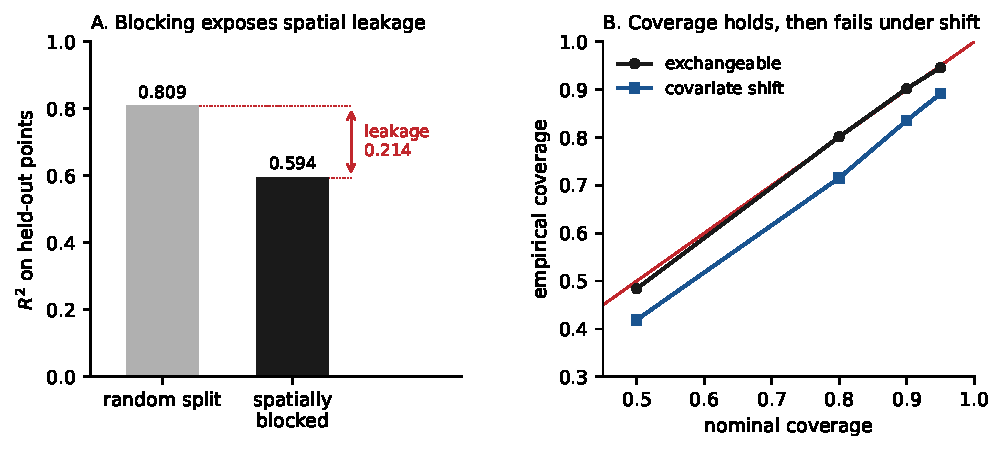
\includegraphics[width=0.95\textwidth]{../figures/fig3_simulation.pdf}
\caption{Simulation checks. \textbf{A}: points carry an unobserved short-range
field absent from the covariates, so leakage exists by construction. A random
split scores $R^2 = 0.809$ and a spatially blocked split scores $0.594$, a gap
of $0.214$, which is the leakage the blocking is meant to expose. \textbf{B}:
split conformal calibrated on one distribution and tested on the same one
attains its nominal level, and loses coverage when the test distribution is
shifted. At nominal 90\% coverage is $0.902$ under exchangeability and $0.836$
under shift.}
\label{fig:sim}
\end{figure}

\paragraph{Does the blocking expose leakage?} Points are placed on a jittered
grid. The observed covariates are smooth, long-wavelength spatial fields, so a
point's covariate vector effectively encodes where it is. The target adds a
short-wavelength field that is \emph{not} among the covariates, standing in for
local conditions no covariate set measures.

Under a random split a flexible model can locate a test point from its
covariates, find its near neighbours in the training set, and recover their
unobserved local conditions. Under a blocked split those neighbours are absent.
Leakage is therefore present by construction, and a blocking scheme that fails
to reveal it is not working. The gap is $0.214$ (Figure~\ref{fig:sim}A), which
is the same order as the gaps we observe per country on the real data, 0.070 to
0.370.

\paragraph{Does coverage behave as the theory says?} A model is fitted, then
calibrated on data from one distribution and tested twice: once on data from
that same distribution, and once on data whose covariates are shifted. Noise is
heteroscedastic, so a constant-width interval is not automatically correct and
the calibration set has to do real work.

Coverage attains its nominal level when calibration and test data are
exchangeable, which is what the guarantee promises, and falls when they are not,
which is what the guarantee permits (Figure~\ref{fig:sim}B). This is the
mechanism the paper goes on to look for across a national border, demonstrated
where the shift is imposed rather than inferred.

Neither check validates the finding. They establish that the instruments respond
as intended to effects of known sign and rough magnitude, so that a null result
on the real data can be read as evidence about the data rather than as a silent
failure of the measurement.

\subsection{Sanity gate}

Before any transfer claim we required the pipeline to reproduce an in-country
accuracy figure consistent with published work, with bands fixed in advance.
Pooled in-country blocked $R^2$ was 0.746, above the original ceiling of 0.70.
That ceiling was a proxy for spatial leakage, adopted when no direct test was
available. Three direct tests were then run and none supported leakage: $R^2$
falls only from 0.746 to 0.706 as block size increases sixfold from 110\,km to
660\,km; leave-one-country-out, which removes every spatial neighbour, gives
0.723; and no block was split across folds. The ceiling was also benchmarked
against held-out-country CNN results, while the gate measures in-country blocked
prediction, whose published comparator is $R^2 = 0.69$.

We amended the upper band after seeing 0.746, and the amendment says so. The
band now passes results between 0.70 and 0.85 only when the three diagnostics
are run and reported, and the implementation computes them rather than accepting
an assertion. The original band and the original failure remain in the record.

We also validated the covariate extraction against the DHS Spatial Data
Repository's independently computed cluster covariates. Agreement was moderate
(Spearman 0.727 to 0.963 on nightlights) and below our pre-registered threshold
of 0.90. We report this as a failure. Two internal checks bound its
interpretation: our WorldPop and GHSL summaries, which come from independent
products through the same buffers and code, agree at Spearman 0.907 to 0.951 in
all twelve countries, which is inconsistent with broken buffer geometry or a
broken cluster join; and the DHS composite carries no year, while our extraction
is matched to survey year.

\section{Results}
\label{sec:res}

\subsection{Point accuracy transfers}

\begin{table}[t]
\centering
\small
\begin{tabular}{lr}
\toprule
Setting & $R^2$ \\
\midrule
In-country, random split (naive) & 0.783 \\
In-country, spatially blocked & 0.746 \\
Out-of-country, leave-one-country-out (mean of 11) & 0.723 \\
Target country, The Gambia & 0.673 \\
\bottomrule
\end{tabular}
\caption{Point accuracy. The gap between random and blocked in-country splits
quantifies spatial leakage in the naive estimate.}
\label{tab:r2}
\end{table}

\begin{figure}[t]
\centering
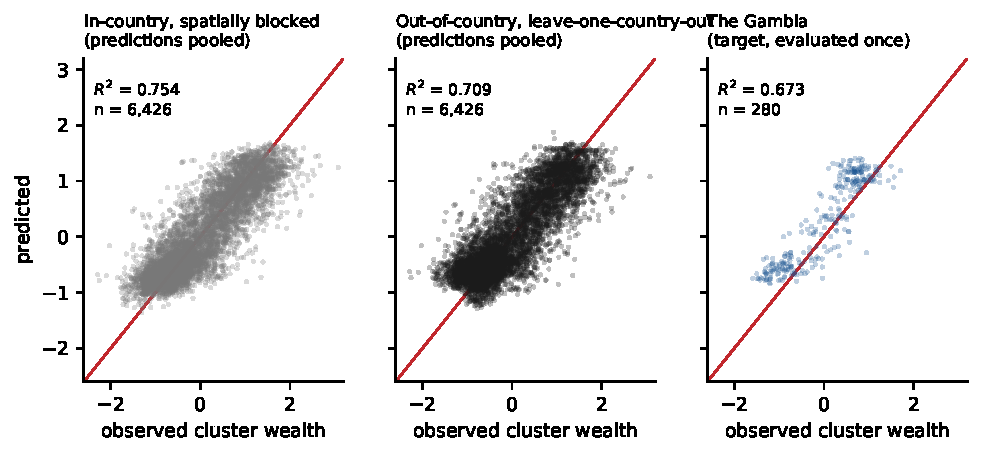
\includegraphics[width=\textwidth]{../figures/fig5_predicted_observed.pdf}
\caption{Predicted against observed cluster wealth, with the identity line in
red. The target panel reproduces the registered evaluation exactly, fitted on
folds 3 to 9 with folds 0 to 2 reserved for conformal calibration; fitting on
all eleven training countries instead would give 0.696. The first two panels
pool predictions across folds and countries, so their $R^2$ differs slightly
from Table~\ref{tab:r2}, which reports means across folds and across countries
respectively. Predictions are visibly compressed toward the mean in all three
panels, over-predicting the poorest clusters and under-predicting the richest,
which is the pattern \citet{corral2025} report for point estimates in
unsurveyed areas.}
\label{fig:predobs}
\end{figure}

H1 predicted an out-of-country drop of roughly a third. The observed drop from
in-country blocked to leave-one-country-out is 0.023, about three per cent
(Table~\ref{tab:r2}). H1 is falsified. This is consistent with \citet{yeh2020},
who already report that point accuracy survives a border.

\subsection{Mean coverage transfers}

\begin{table}[t]
\centering
\small
\begin{tabular}{lrrrrr}
\toprule
& \multicolumn{3}{c}{Training pool (mean of 11)} & \multicolumn{2}{c}{The Gambia} \\
\cmidrule(lr){2-4}\cmidrule(lr){5-6}
Nominal & In-country & Out-of-country & Shortfall & Split & CQR \\
\midrule
0.50 & 0.524 & 0.491 & 0.033 & 0.371 & 0.475 \\
0.80 & 0.825 & 0.785 & 0.041 & 0.704 & 0.775 \\
0.90 & 0.913 & 0.887 & 0.026 & 0.893 & 0.896 \\
0.95 & 0.956 & 0.943 & 0.013 & 0.961 & 0.968 \\
\bottomrule
\end{tabular}
\caption{Empirical coverage of conformal prediction intervals. Training-pool
columns use split conformal. Gambian columns are the single pre-registered
evaluation.}
\label{tab:cov}
\end{table}

H2, the central claim, predicted that a nominal 90\% interval would cover
substantially less than 90\% out-of-country. It covered 88.7\% across the eleven
held-out training countries and 89.3\% on The Gambia (Table~\ref{tab:cov}). H2 is
not supported.

The pre-registered target test, H4, asked whether Gambian coverage at nominal
90\% would fall outside $[0.865, 0.935]$, the two-sided 95\% binomial interval at
$n = 280$ under exactly nominal coverage. It did not ($0.893$, $z = -0.40$). H4 is
not confirmed. The test has power 0.529 against a false positive rate of 0.050,
stated in advance, so this null is weak evidence and should not be read as
evidence that coverage is reliable.

\subsection{Correlation alignment does not help}

H3 predicted that domain adaptation would improve point accuracy while leaving
calibration unrepaired. CORAL \citep{sun2016} degraded point accuracy, from
$R^2 = 0.709$ to $0.646$ out-of-country, and worsened the interval score for
both conformal methods.

The baseline here is 0.709 rather than the 0.723 in Table~\ref{tab:r2} because
the two are computed on different training sets. Table~\ref{tab:r2} fits each
leave-one-country-out model on all ten remaining countries. The conformal
experiments must reserve part of the source data to calibrate on, so they fit
on five of ten spatial folds and hold three for calibration, which is roughly
half the data and costs about 0.014 in $R^2$. Both figures are reported rather
than reconciled to one, since each is the correct baseline for its own
comparison. The premise fails, so the comparison H3 proposed cannot be made. The
reasoning behind H3 is nonetheless consistent with what we observe: aligning
feature distributions contains no mechanism acting on interval width, and the
dispersion of coverage across countries was unchanged (0.053 to 0.055 for split
conformal, 0.060 to 0.062 for CQR). Only second-moment alignment was tested; the
adversarial variant named in the protocol was not run.

\subsection{The average conceals a wide per-country spread}
\label{sec:disp}

The following was found after the pre-registered questions had been answered.
It is post-hoc in origin, and the evidence for it is nonetheless far stronger
than for anything the registered hypotheses addressed.


At nominal 90\%, out-of-country coverage ranged from 0.821 (Mauritania) to
0.979 (Togo), with standard deviation 0.053 against 0.019 in-country
(Figures~\ref{fig:map} and~\ref{fig:heat}). Nine of eleven countries fall
outside an 88 to 92\% band.

The dispersion is not a feature of one nominal level. Table~\ref{tab:disp}
tests, at each level, whether the eleven observed coverages are consistent with
every country having exactly nominal coverage and differing only by sampling at
that country's cluster count. They are not, at any level, by a wide margin.

\begin{table}[t]
\centering
\small
\begin{tabular}{lrrrrl}
\toprule
Nominal & sd across countries & binomial sd & ratio & $\chi^2_{10}$ & $p$ \\
\midrule
50\% & 0.1108 & 0.0237 & 4.68 & 273.1 & $<10^{-50}$ \\
80\% & 0.0889 & 0.0189 & 4.70 & 269.9 & $<10^{-50}$ \\
90\% & 0.0531 & 0.0142 & 3.74 & 195.1 & $<10^{-35}$ \\
95\% & 0.0289 & 0.0103 & 2.80 & 108.9 & $<10^{-17}$ \\
\bottomrule
\end{tabular}
\caption{Between-country dispersion of out-of-country coverage, split
conformal. The binomial column is the standard deviation expected if every
country's true coverage were exactly nominal and the only variation were
sampling at that country's cluster count. Observed dispersion exceeds it by a
factor of 2.8 to 4.7 at every level.}
\label{tab:disp}
\end{table}

This is the clearest empirical result in the paper and the one with a direct
practical consequence. A mean of 88.7\% against a nominal 90\% suggests these
intervals can be used as stated. Per country they cannot: the same procedure
that covers 82\% of Mauritanian clusters covers 98\% of Togolese ones, and
nothing observable in advance separates the two cases. A user deploys to one
country, and the mean over eleven is not the quantity they need.

The dispersion also grows as the nominal level falls, from a ratio of 2.80 at
95\% to 4.68 at 50\%. Intervals are least trustworthy where they are narrowest,
which is the regime a decision rule with a moderate threshold would operate in.


\begin{figure}[t]
\centering
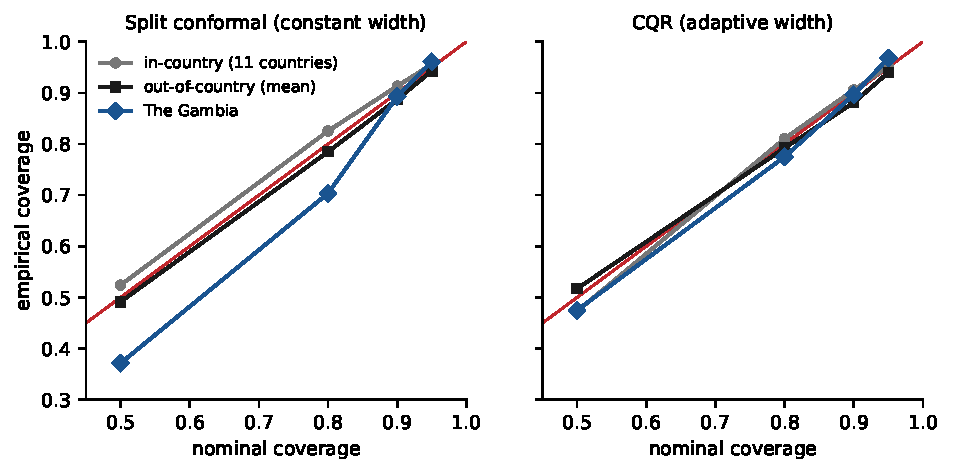
\includegraphics[width=0.95\textwidth]{../figures/fig2_calibration_curves.pdf}
\caption{Calibration curves. The two conformal methods agree closely in-domain
and out-of-domain on the training pool. On The Gambia they separate at the lower
nominal levels: constant-width split conformal undercovers at nominal 50\% and
80\% while adaptive CQR does not. Coverage that fails in the middle of the
distribution and holds in the tails is characteristic of a width of the wrong
shape rather than one uniformly too small.}
\label{fig:calib}
\end{figure}
\begin{figure}[t]
\centering
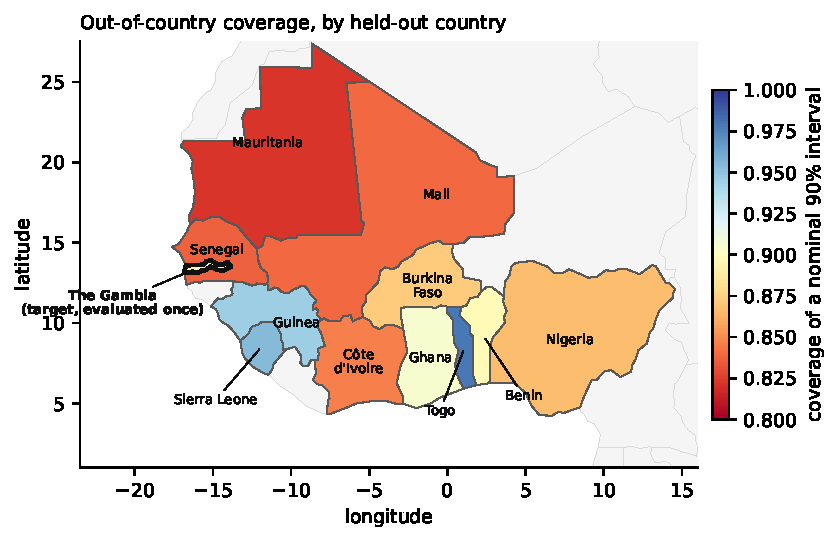
\includegraphics[width=0.8\textwidth]{../figures/fig4_study_area.pdf}
\caption{The twelve surveys, shaded by out-of-country coverage of a nominal
90\% interval. The Gambia is outlined and was evaluated once. The failures are
not uniformly distributed: the Sahelian countries at the top of the map
undercover and the wetter coastal countries overcover. That apparent gradient
was noticed by inspecting this figure and is treated as a lead in
Section~\ref{sec:disc}, not as a result.}
\label{fig:map}
\end{figure}

\begin{figure}[t]
\centering
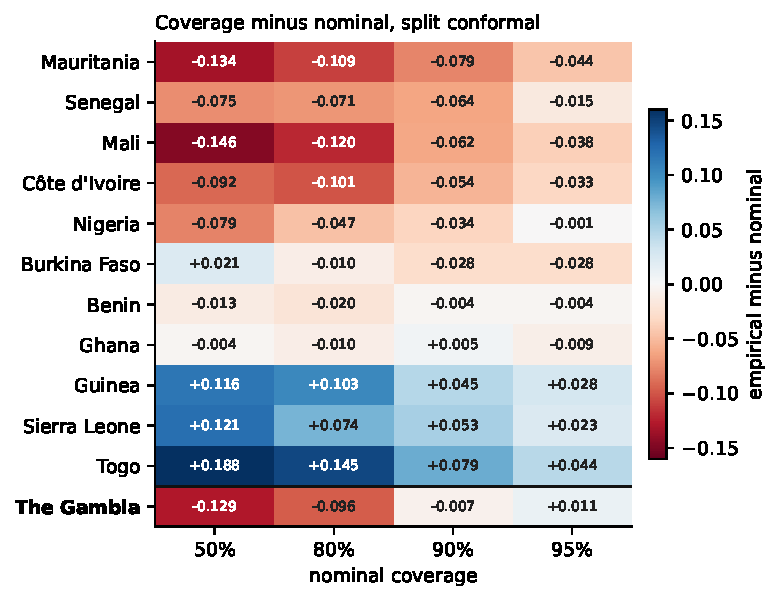
\includegraphics[width=0.72\textwidth]{../figures/fig6_coverage_heatmap.pdf}
\caption{Empirical minus nominal coverage, split conformal, by country and
nominal level. Both post-hoc observations are visible at once. Reading down a
column gives the dispersion across countries, from Mali at $-0.146$ to Togo at
$+0.188$ at nominal 50\%. Reading along a row gives the level dependence: for
almost every country the deviation shrinks as the nominal level rises. The
Gambia, below the rule, shows that pattern clearly, at $-0.129$, $-0.096$,
$-0.007$ and $+0.011$.}
\label{fig:heat}
\end{figure}

\subsection{An apparent shape effect, tested and withdrawn}

On The Gambia, split conformal undercovered at nominal 50\% ($0.371$) and 80\%
($0.704$) while holding at 90\% and 95\%, and CQR did not
(Figure~\ref{fig:heat}, bottom row). Against binomial sampling those deviations
are $z = -4.30$ and $z = -4.03$. Coverage that fails in the middle of the
distribution and holds in the tails is characteristic of an interval of the
wrong shape rather than one uniformly too narrow, which is the axis separating
constant-width from adaptive methods, and both were included in advance for
exactly this comparison.

We tested it and it does not survive. Two checks, both reported.

\paragraph{It does not replicate across the training pool.} Comparing the
absolute deviation from nominal for split conformal against CQR, country by
country, the two are indistinguishable at every level: mean absolute deviation
0.090 against 0.098 at nominal 50\%, 0.074 against 0.077 at 80\%, 0.046 against
0.050 at 90\%, and 0.024 against 0.026 at 95\%. A Wilcoxon signed-rank test over
the eleven countries gives $p$ between 0.37 and 0.90 at every level, and split
conformal is the closer of the two more often than not. If constant width were
the problem, this is where it would appear.

\paragraph{The Gambian deviations are ordinary once the right reference is
used.} The $z$ values above compare the target against binomial sampling, which
presumes every country's coverage is exactly nominal. Table~\ref{tab:disp} shows
that presumption fails by a factor of three to five. Measured against the
observed between-country distribution instead, The Gambia sits at $z = -1.08$,
$-0.91$, $+0.11$ and $+0.62$ across the four levels. It is a typical draw.

The apparent shape effect was therefore the dispersion of
Section~\ref{sec:disp} seen through the wrong reference distribution, at the
level where that dispersion is largest. We report it because it was a
pre-specified secondary comparison and because the reasoning behind it is sound
in general. It is simply not what these data show, and on this evidence the
choice between constant-width and adaptive conformal intervals is not the lever
that matters.


\section{Discussion}
\label{sec:disc}

Our pre-registered expectations were that transfer would be harmful and that
uncertainty would be the first thing to break. Neither held. Across eleven
country pairs and one held-out target, point accuracy degraded by about three
per cent and mean interval coverage stayed within about one and a half points of
nominal.

We take the practical implication to be that these models transfer better than
caution about distribution shift would suggest, at least within a region of
neighbouring countries with a common survey instrument.

That conclusion should be read against \citet{adjei2026}, who measure conformal
coverage on an African satellite product under spatial shift and find it falls
to 65.3\% against a 90\% target. Coverage clearly can collapse in this setting,
so the question is what differs here. Three things plausibly do. Their shift is
between regions of a continent while ours is between adjacent countries sharing
a survey instrument, so the covariate distributions are closer. Their label is
a physical concentration with an absolute scale, while ours is standardised
within each country by construction, which removes level differences from the
label before any model sees it. And their in-domain accuracy is much lower
($R^2 = 0.134$ under spatial cross-validation against our 0.746), so their
intervals are calibrated on residuals from a weaker model. We cannot separate
these with the data here, and the comparison is a reason to treat our result as
specific to this setting rather than as a general finding about conformal
prediction under geographic shift.

It also suggests the two results are less different than they appear. Adjei et
al. report one number for one region; we report eleven, and ours span 0.821 to
0.979. Their 65.3\% is outside our range, so the difference is real, but a study
reporting only our mean of 0.887 would have concealed a spread wide enough that
a single unlucky country could look like their case. The reconciliation may be
less about our setting being benign than about how much a single coverage figure
can hide, which is the point of Table~\ref{tab:disp}.

\subsection{Limitations}

Our source countries are neighbours of the target and share a survey
instrument, so this measures transfer under a modest distribution shift.
Transfer to a more distant region would plausibly be worse, making these results
a lower bound on the problem.

The wealth index is an asset index standardised within country, not a measure of
consumption or income, and its cross-country comparability is assumed rather
than demonstrated. Mauritania sampled about ten households per cluster where
other surveys sampled twenty to thirty, so its cluster means carry roughly 1.6
times the label noise, and this is correlated with country. Land cover comes
from a single 2021 epoch applied to every survey year, which for Togo 2014 is an
eight-year gap. The cross-check against DHS's own covariate extraction did not
reach our pre-registered agreement threshold.

The target-country test had 53\% power. This is a consequence of having one
target country with 280 clusters and was stated before the test was run. A study
designed to test the dispersion observation would use many countries and every
nominal level rather than a single draw.

\subsection{A geographic pattern in the failures}

Figure~\ref{fig:map} suggests the coverage failures are not scattered at
random. The three driest, most northerly countries undercover, Mauritania at
0.821, Senegal at 0.836 and Mali at 0.838, while three of the wetter coastal
countries overcover, Togo at 0.979, Sierra Leone at 0.953 and Guinea at 0.945.

Tested after the fact, country mean latitude correlates with coverage at
Spearman $\rho = -0.564$ ($p = 0.071$) and mean annual rainfall at
$\rho = 0.655$ ($p = 0.029$). Two things make this weak evidence and both are
stated rather than left for a reader to notice. The pattern was found by
looking at the map, and the tests were run afterwards on the same eleven
numbers that suggested it. Two covariates were tried, so the smaller $p$ value
should be read with that in mind, and the rank test on latitude does not reach
conventional significance in any case.

We report it because it is a specific, testable proposition for a study
designed around it, and because a reader looking at Figure~\ref{fig:map} would
see it anyway. It is not a finding of this paper.

\subsection{Future work}

The obvious next question is what predicts a country's coverage. Dispersion is
established here, but nothing in this design explains it, and a user needs to
know in advance whether the country in front of them is a Mauritania or a Togo.
The geographic gradient above is one candidate. Covariate shift measured
directly between source and target, as \citet{adjei2026} do, is a better one,
because it is computable without any target labels and is therefore available at
deployment time. Testing whether a shift statistic predicts coverage loss across
countries would turn an observed spread into something actionable, and it is a
design with real power because every country supplies a point.

The second question is what to do about it. Weighted conformal prediction
\citep{tibshirani2019} recovers coverage under covariate shift when the density
ratio between source and target can be estimated. We deliberately used the
unweighted method, since the question here was what happens to the guarantee as
it is ordinarily applied. Whether the weighted correction narrows the spread in
Table~\ref{tab:disp} is a direct and answerable follow-up.

We do not propose further work on interval shape. The comparison was made, it
did not replicate, and the reference-distribution error that produced it is
explained above.

\section{Conclusion}

We pre-registered four hypotheses about how satellite-based poverty models fail
across a national border and found no support for any of them. Point accuracy
and mean interval coverage both transferred, and correlation alignment made
accuracy worse.

The hypotheses were aimed at the wrong quantity. Averaged over eleven held-out
countries these intervals behave close to their stated level, which is why every
prediction about the average failed. Per country they do not: coverage is
dispersed by three to five times what sampling permits at every nominal level,
and the spread widens as the interval narrows. That dispersion is not a
secondary caveat to a null result. It is the finding, it is measured on eleven
independent country pairs rather than asserted, and it bears directly on use,
because these maps are deployed one country at a time and the mean over eleven
is not what a user gets.

We also report a secondary comparison that did not survive testing. An apparent
failure of constant-width intervals on the target dissolved once the eleven
training countries were checked and once the deviations were measured against
the observed between-country distribution rather than against binomial sampling.
It is described rather than omitted, because the reference-distribution error
that produced it is easy to make and the correction is the substantive point.

\section*{Data and code availability}

All code is available at \url{https://github.com/Balisa50/gambia-poverty-transfer},
including the protocol, the dated amendments, the pre-registration and the
evaluation script. DHS microdata cannot be redistributed under the terms of use
and is not included; it is available on application at
\url{https://dhsprogram.com}. All covariates are from open sources requiring no
application.

\section*{Acknowledgements}

This work uses data from The DHS Program. The author thanks the DHS Program for
access to the survey and geographic datasets.

\begin{thebibliography}{99}
\setlength{\itemsep}{2pt}

\bibitem[Adjei et al.(2026)]{adjei2026}
Y.~O. Adjei, D.~Opoku, E.~Abotsi, K.~O. Amanqua, O.~Kornyo, E.~Soglo-Ahianyo,
and C.~A. Abbey.
\newblock Conformal PM2.5 mapping under spatial covariate shift: satellite-reanalysis
fusion for Africa's green industrial transition.
\newblock arXiv:2604.22787, 2026.
\newblock \url{https://arxiv.org/abs/2604.22787}

\bibitem[Barber et al.(2023)]{barber2023}
R.~F. Barber, E.~J. Cand\`es, A.~Ramdas, and R.~J. Tibshirani.
\newblock Conformal prediction beyond exchangeability.
\newblock \emph{The Annals of Statistics}, 51(2):816--845, 2023.
\newblock \url{https://doi.org/10.1214/23-AOS2276}

\bibitem[Blumenstock et al.(2015)]{blumenstock2015}
J.~Blumenstock, G.~Cadamuro, and R.~On.
\newblock Predicting poverty and wealth from mobile phone metadata.
\newblock \emph{Science}, 350(6264):1073--1076, 2015.
\newblock \url{https://doi.org/10.1126/science.aac4420}

\bibitem[Burgert et al.(2013)]{burgert2013}
C.~R. Burgert, J.~Colston, T.~Roy, and B.~Zachary.
\newblock Geographic displacement procedure and georeferenced data release
policy for the Demographic and Health Surveys.
\newblock DHS Spatial Analysis Reports No.~7. ICF International, Calverton,
Maryland, 2013.

\bibitem[Chi et al.(2022)]{chi2022}
G.~Chi, H.~Fang, S.~Chatterjee, and J.~E. Blumenstock.
\newblock Microestimates of wealth for all low- and middle-income countries.
\newblock \emph{Proceedings of the National Academy of Sciences},
119(3):e2113658119, 2022.
\newblock \url{https://doi.org/10.1073/pnas.2113658119}

\bibitem[Kakooei and Daoud(2024)]{kakooei2024}
M.~Kakooei and A.~Daoud.
\newblock Increasing the confidence of predictive uncertainty: earth
observations and deep learning for poverty estimation.
\newblock \emph{IEEE Transactions on Geoscience and Remote Sensing}, 62, 2024.
\newblock \url{https://doi.org/10.1109/TGRS.2024.3392605}

\bibitem[Masaki et al.(2020)]{masaki2020}
T.~Masaki, D.~Newhouse, A.~R. Silwal, A.~Bedada, and R.~Engstrom.
\newblock Small area estimation of non-monetary poverty with geospatial data.
\newblock Policy Research Working Paper 9383. World Bank, Washington, DC, 2020.
\newblock \url{https://doi.org/10.1596/1813-9450-9383}

\bibitem[Newhouse(2023)]{newhouse2023}
D.~Newhouse.
\newblock Small area estimation of poverty and wealth using geospatial data:
what have we learned so far?
\newblock Policy Research Working Paper 10512. World Bank, Washington, DC, 2023.
\newblock \url{https://doi.org/10.1596/1813-9450-10512}

\bibitem[Olanrewaju and Adebayo(2026)]{olanrewaju2026}
A.-S. Olanrewaju and S.~Adebayo.
\newblock Measuring subnational welfare across sub-Saharan Africa: reproducible
relative-wealth estimates from open satellite data.
\newblock SSRN working paper 7086839, 2026.
\newblock \url{https://papers.ssrn.com/sol3/papers.cfm?abstract_id=7086839}

\bibitem[Permatasari and Ubaidillah(2025)]{permatasari2025}
N.~Permatasari and A.~Ubaidillah.
\newblock Small area estimation of poverty using remote sensing data.
\newblock \emph{Statistical Journal of the IAOS}, 41, 2025.
\newblock \url{https://doi.org/10.1177/18747655241308390}

\bibitem[Corral et al.(2025)]{corral2025}
P.~Corral, H.~Henderson, and S.~Segovia.
\newblock Poverty mapping in the age of machine learning.
\newblock \emph{Journal of Development Economics}, 172:103377, 2025.
\newblock \url{https://doi.org/10.1016/j.jdeveco.2024.103377}

\bibitem[Lee and Braithwaite(2022)]{lee2022}
K.~Lee and J.~Braithwaite.
\newblock High-resolution poverty maps in sub-Saharan Africa.
\newblock \emph{World Development}, 159:106028, 2022.
\newblock \url{https://doi.org/10.1016/j.worlddev.2022.106028}

\bibitem[Jean et al.(2016)]{jean2016}
N.~Jean, M.~Burke, M.~Xie, W.~M. Davis, D.~B. Lobell, and S.~Ermon.
\newblock Combining satellite imagery and machine learning to predict poverty.
\newblock \emph{Science}, 353(6301):790--794, 2016.
\newblock \url{https://doi.org/10.1126/science.aaf7894}

\bibitem[Ploton et al.(2020)]{ploton2020}
P.~Ploton, F.~Mortier, M.~R\'ejou-M\'echain, N.~Barbier, N.~Picard, V.~Rossi,
et al.
\newblock Spatial validation reveals poor predictive performance of large-scale
ecological mapping models.
\newblock \emph{Nature Communications}, 11(1):4540, 2020.
\newblock \url{https://doi.org/10.1038/s41467-020-18321-y}

\bibitem[Roberts et al.(2017)]{roberts2017}
D.~R. Roberts, V.~Bahn, S.~Ciuti, M.~S. Boyce, J.~Elith, G.~Guillera-Arroita,
et al.
\newblock Cross-validation strategies for data with temporal, spatial,
hierarchical, or phylogenetic structure.
\newblock \emph{Ecography}, 40(8):913--929, 2017.
\newblock \url{https://doi.org/10.1111/ecog.02881}

\bibitem[Romano et al.(2019)]{romano2019}
Y.~Romano, E.~Patterson, and E.~J. Cand\`es.
\newblock Conformalized quantile regression.
\newblock In \emph{Advances in Neural Information Processing Systems 32
(NeurIPS 2019)}, pages 3543--3553, 2019.

\bibitem[Smythe and Blumenstock(2022)]{smythe2022}
I.~S. Smythe and J.~E. Blumenstock.
\newblock Geographic microtargeting of social assistance with high-resolution
poverty maps.
\newblock \emph{Proceedings of the National Academy of Sciences},
119(32):e2120025119, 2022.
\newblock \url{https://doi.org/10.1073/pnas.2120025119}

\bibitem[Sun and Saenko(2016)]{sun2016}
B.~Sun and K.~Saenko.
\newblock Deep CORAL: correlation alignment for deep domain adaptation.
\newblock In \emph{Computer Vision -- ECCV 2016 Workshops}, volume 9915 of
\emph{Lecture Notes in Computer Science}, pages 443--450. Springer, 2016.
\newblock \url{https://doi.org/10.1007/978-3-319-49409-8_35}

\bibitem[Tibshirani et al.(2019)]{tibshirani2019}
R.~J. Tibshirani, R.~F. Barber, E.~J. Cand\`es, and A.~Ramdas.
\newblock Conformal prediction under covariate shift.
\newblock In \emph{Advances in Neural Information Processing Systems 32
(NeurIPS 2019)}, pages 2530--2540, 2019.

\bibitem[Vovk et al.(2005)]{vovk2005}
V.~Vovk, A.~Gammerman, and G.~Shafer.
\newblock \emph{Algorithmic Learning in a Random World}.
\newblock Springer, New York, 2005.

\bibitem[Yeh et al.(2020)]{yeh2020}
C.~Yeh, A.~Perez, A.~Driscoll, G.~Azzari, Z.~Tang, D.~Lobell, S.~Ermon, and
M.~Burke.
\newblock Using publicly available satellite imagery and deep learning to
understand economic well-being in Africa.
\newblock \emph{Nature Communications}, 11(1):2583, 2020.
\newblock \url{https://doi.org/10.1038/s41467-020-16185-w}

\end{thebibliography}

\end{document}
